% put all Mike's macros in and begin document
\documentclass[pdftex]{article}
\usepackage[pdftex]{graphics}
\usepackage{subfigure}
\usepackage{hhline}
\usepackage[usenames,dvipsnames]{color}
\usepackage{colortbl}
\usepackage[screen,pdftex]{mcdlecture}
\newcommand{\bs}{\relax}
\newcommand{\es}{\newpage}
\fboxsep=.01\textwidth \fboxrule=1pt
\newsavebox{\savepar}
\newenvironment{boxit}{\begin{lrbox}{\savepar}
    \begin{minipage}[b]{0.975\textwidth}}
    {\end{minipage}\end{lrbox}\framebox{\usebox{\savepar}}}


%%%%%%%%%%%%%%%%%%%%%%%%%%%%%%%%%%%%%%%%%%%%%%%%%%%%%%%%%%
%% THE FOLLOWING ARE THINGS THAT WE MIGHT CHANGE FROM YEAR TO YEAR OR
%% VENUE TO VENUE
    \lhead{MCMC in Statistical Genetics}
    \lfoot{Dr Eric C. Anderson and Dr Matthew Stephens}
%	\lfoot{Dr Eric C. Anderson and Dr John Novembre}
%    \rfoot{UW - Summer Institute, July 2013}
%	 \rfoot{Edinburgh - European Institute, June 2012}
\rfoot{Brazil - Summer Institute, February 2014}

% on this one, be sure to update the venue and the module number
%\newcommand{\coursetitlepage}{European Institute in Statistical Genetics
%\newcommand{\coursetitlepage}{Summer Institute in Statistical Genetics
\newcommand{\coursetitlepage}{Brazilian Edition of the Summer \\Institute in Statistical Genetics

Module 9:

MCMC for Genetics}

%% Then update the schedule.  Note that I have broken that
%% out into a separate file like: schedule_table_edinburgh2012.tex
%% which is input in Overview.tex

%% Then be sure to change any time-sensitive events in the 
%% probability discussion in Matthew's first lecture.

%% And also update "structure_fun" link to my wiki to the right
%% year and venue.
%%%%%%%%%%%%%%%%%%%%%%%%%%%%%%%%%%%%%%%%%%%%%%%%%%%%%%%%%%


\begin{document}

\DeclareGraphicsExtensions{.jpg,.pdf,.png}%



%% Eric added a few things:
% some commands that Eric made for making a title while starting
% a new lecture and for making titles of new slides.
\newcommand{\newlecture}[1]{\newpage\begin{center}\section*{#1}\end{center}}
\newcommand{\newslide}[1]{\newpage\subsection*{#1: \hfil}}
 \newcommand{\Exp}{\Bbb{E}}
 \newcommand{\Var}{{\mathrm{Var}}}
 %% Some pretty etc.'s, etc...
\newcommand{\cf}{{\em cf.}}
\newcommand{\eg}{{\em e.g.},}
\newcommand{\ie}{{\em i.e.},}
\newcommand{\etal}{{\em et al.}\ }
\newcommand{\etc}{{\em etc.}}

%% some handy things for making bold math
\def\bm#1{\mathpalette\bmstyle{#1}}
\def\bmstyle#1#2{\mbox{\boldmath$#1#2$}}
\newcommand{\thh}{^\mathrm{th}}
\newcommand{\bpi}{{\pi}}
\newcommand{\mP}{\mathbf{P}}

\rhead{Session 2 - \thepage}




% each \include command puts a new file in.

% to make typesetting faster while working on a single
% section, but still have the appropriate page numbering
% and references, use the \includeonly command



\newlecture{Monte Carlo \\ (No Markov Chains\ldots Yet)}
Goals of this lecture:
\begin{itemize}
\item Define the Monte Carlo method generally
\item Explain why Monte Carlo is useful
\item Understand variance of Monte Carlo estimators
\end{itemize}
all without talking about Markov chains\ldots

\newslide{The origin of Monte Carlo}

First Reference:

\textsc{Metropolis, N. and S. Ulam.}  1949.  The Monte Carlo method.  {\em Journal of the American Statistical Association}. 44:335--341.

The name ``Monte Carlo" was coined originally by John von Neumann and Stanislaw Ulam who used the phrase as a code word at Los Alamos for their simulation-based computational methods used to solve the problem of initiating fusion in a thermonuclear bomb. 

Earlier examples exist.  (for example, the Comte de Buffon and his needle in the mid-1700's).  

With computer power increasing all the time, Monte Carlo methods are more widespread than ever, and are used in a wide range of applications, most of them of a more humanitarian bent than bomb design.    

\newpage

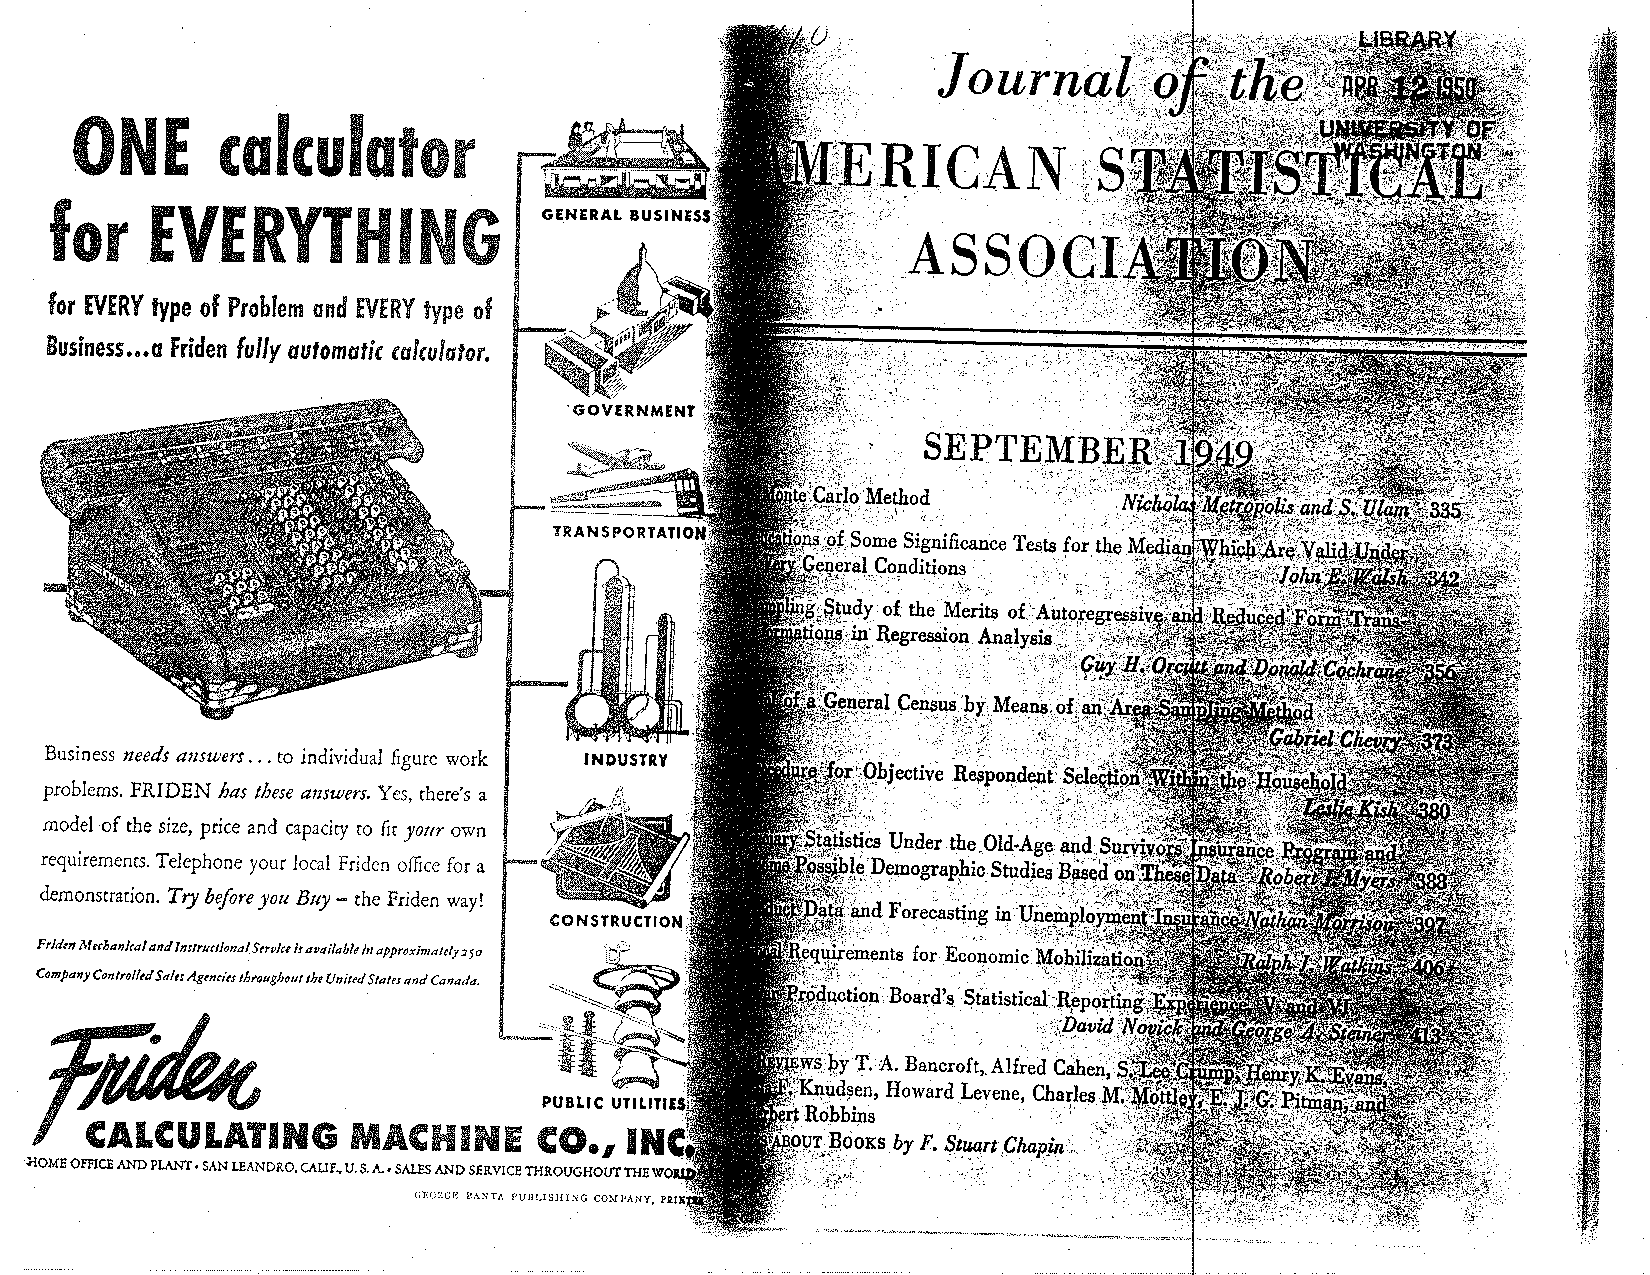
\includegraphics[width=\textwidth]{illus/JASA_MC_Article_Adding_Machine.pdf}
 

\newslide{In search of a definition for Monte Carlo}
There are few concise, yet general definitions in the literature.  Some, like Ripley (1987) reserve ``Monte Carlo" only for ``Monte Carlo Integration" and ``Monte Carlo Tests," and refer to all else as ``stochastic simulation."

Others use Monte Carlo to refer specifically to the generation of pseudo-random numbers:
   
\begin{minipage}{.60\textwidth }
{\sl ``One way to increase our confidence in the methods we use is to test models and methods on sets of data in which we know exactly what is happening\ldots A useful method for generating such data is called the Monte Carlo method.\ldots The Monte Carlo method uses random number generators for the construction of data."}
\end{minipage}
\hfill
\begin{minipage}{.35\textwidth }
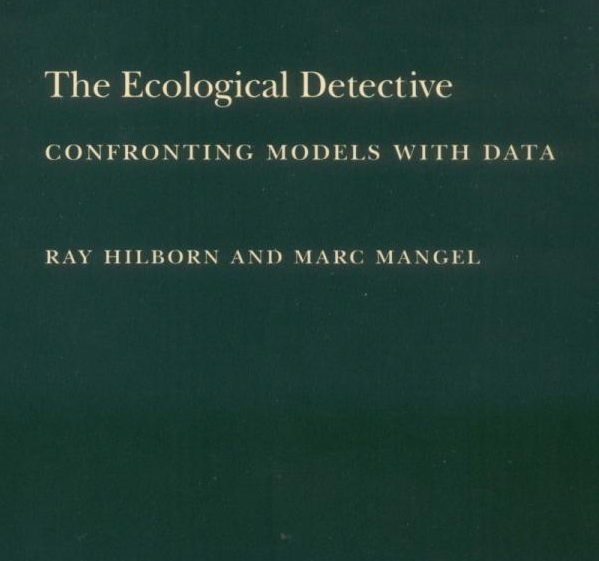
\includegraphics[width=\textwidth]{illus/ecodetect}
\end{minipage}


\newslide{A general definition of the Monte Carlo method}
\textsc{definition}: {\sl Monte Carlo is the art of approximating an expectation by the sample mean of a function of simulated random variables.}

This definition is general enough to encompass everything that has been called ``Monte Carlo," yet also makes clear its essence in familiar terms: Monte Carlo is about invoking laws of large numbers to approximate expectations.

\textsc{review:} {\sl Expectations}.
\[
\Exp[g(X)]= \int_{x\in\mathcal{X}} g(x)f_X(x)dx~~~~~~~~
\mathrm{or}~~~~~~~
\Exp[g(X)] = \sum_{x\in\mathcal{X}} g(x)f_X(x)
\]
\textsc{review:} {\sl Weak Law of Large Numbers}.\\
Let $X_1,X_2,\ldots,X_n$ be iid  r.v.'s with $\Exp|X_i|<\infty$, and $\bar{X}_n = \frac{1}{n}\sum_{1}^nX_i$.  Then 
\[
\lim_{n\rightarrow\infty} P(|\bar{X}_n - \Exp X_i| > \epsilon) = 0~~~~\mathrm{for~any}~\epsilon>0 
\]

\newslide{A Suggestion from the weak law of large numbers:}
Any expectation may be approximated by the sample mean of $n$ random variables (and it will work better if $n$ is large).
\[
	\Exp[g(X)] \approx \frac{1}{n}\sum_{i=1}^n g(x^{(i)})~~~~\mathrm{with}~~~X^{(i)}\sim f_X
\]

\newslide{Why estimating expectations is useful}
Usually, any quantity of interest may be expressed as the expected value of a function of some random variable.  Importantly:
\begin{description}
\item[Probabilities:] 
\[
	P(X\in \mathcal{A}) = \Exp[ I_{\{\mathcal{A}\}}(X)]
\]
where $I_{\{\mathcal{A}\}}(X)$ is the {\em indicator function} taking the value 1 when $X\in\mathcal{A}$ and 0 otherwise.
\item[Integrals:] For a simple example, let $U$ be a uniform r.v. on the interval $[a,b)$ with pdf $f_U(u) = 1/(b-a)$.  Hence 
\[
	\int_a^b q(x)dx = (b-a)\int_a^b q(x)\frac{1}{b-a}dx = (b-a)\Exp[q(U)]
\]
We see here a case where Monte Carlo applies to a purely deterministic problem.
\item[Discrete Sums:] In the same vein as above, just as any integral can be approximated by Monte Carlo, so can any sum. For another simple, uniform example, let $W$ be a discrete random variable that takes all values $w$ in the set $\mathcal{A}$ with equal probability $p$. Then, the sum $\sum_{x\in\mathcal{A}}q(x)$ is easily approximated by Monte Carlo:
\[
	\sum_{x\in\mathcal{A}}q(x)  = {\displaystyle\frac{1}{p}  }
	\sum_{x\in\mathcal{A}}q(x)p = 
	{\displaystyle\frac{1}{p}  }
	\Exp[q(W)].
\]   
This is particularly useful in statistical genetics, because many probabilities of interest may be expressed as an intractable sum over latent variables.
\end{description}

The bottom line is that, since you can cast any quantity as an expectation; you can (in theory) approximate any quantity by Monte Carlo.  In the simplest case, when $X$ is distributed according to $f_X$.  
\[
	\Exp[g(X)] \approx \frac{1}{n}\sum_{i=1}^n g(x^{(i)})~~~~\mathrm{with}~~~X^{(i)}\sim f_X
\]

\newslide{Genetics example I: Estimating probabilities in the Wright-Fisher model}
The Wright-Fisher model underlies most population genetics theory that deals with the descent of genes in a finite population from one generation to the next.

A schematic of its underlying assumptions:
\begin{center}
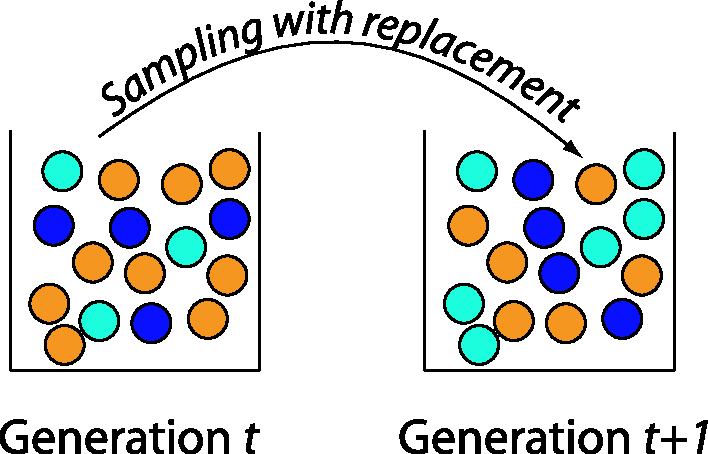
\includegraphics[width=.52\textwidth]{illus/wfmodel.pdf}
\end{center}

\newslide{Genetics example I: Estimating probabilities in the Wright-Fisher model}
Let $X$ be the frequency of the $A$ allele in a Wright-Fisher population of size $2N=200$ after 14 generations of drift, having started from a frequency of 60 out of 200.

The distribution of $X$ can be approximated by simulating $n=50,000$ instances:
\begin{center}
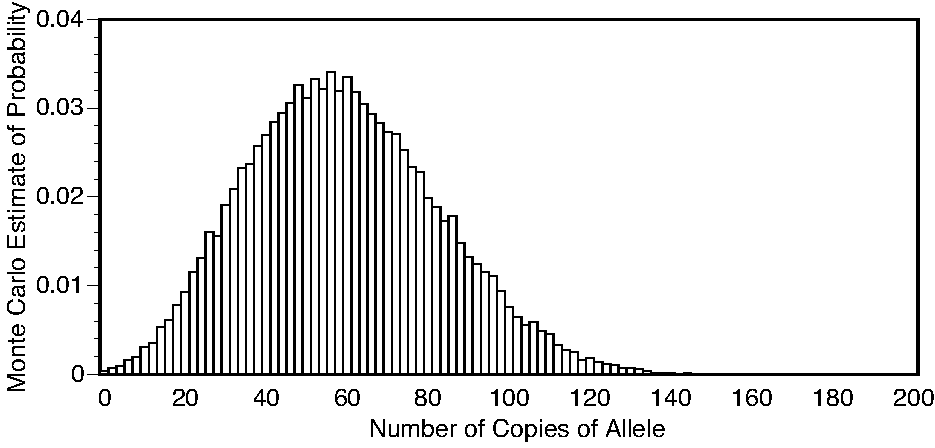
\includegraphics[width=.6\textwidth]{illus/wfhist.pdf}
\end{center} 
Each histogram column is an approximation of an expectation:
\begin{eqnarray}
		P(a\leq X<a+2) & = & \Exp[I_{\{x:a\leq x<a+2\}}(X)] \nonumber  \\
		&\approx & \displaystyle \frac{1}{n}
		\sum_{i=1}^n I_{\{x:a\leq x<a+2\}}(x^{(i)}) \nonumber
\end{eqnarray}
for $a=0,2,\ldots,200$, where each $x^{(i)}$ is an independent realization of the 
number of $A$ alleles at $t=14$ in the Wright-Fisher model.
\newslide{Genetics example II: estimating a sum over latent variables} Wright and McPhee (1925) estimating inbreeding of individuals within cattle pedigrees.
\begin{center}
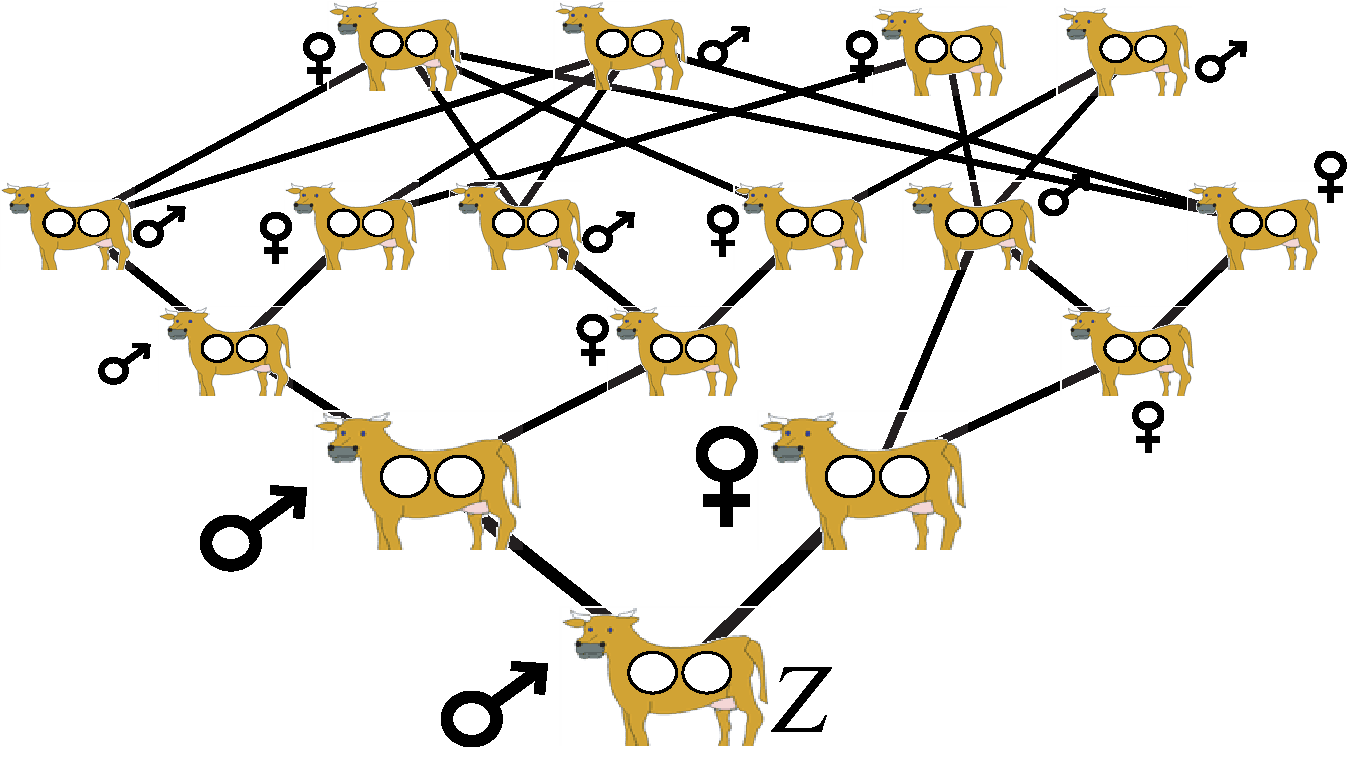
\includegraphics[width=.83\textwidth]{illus/cows.pdf}
\end{center}
In terms of latent variables:
\begin{itemize}
\item The maternal ($m$) and paternal ($p$) genes in individual $z$ are direct descendants from an {\em unobserved} lineage of ancestral gene copies, \ie
\item $A_m = \{a_{m,1}, a_{m,2},\ldots,a_{m,n}\}$ and $A_p = \{a_{p,1}, a_{p,2},\ldots,a_{p,n}\}$
\item The individual is inbred at a locus if the ancestors of the maternal gene and the paternal gene are the same at any point in their lineages, \ie ~if $A_m\cap A_p \neq \emptyset$.
\item The probability that an individual is inbred at a locus is then the sum over latent variables:
\[
	P(\mathrm{inbred}|\mathrm{pedigree}) = \sum_{A_m,A_p} [1-I_{\{\emptyset\}}(A_m \cap A_p )] P(A_m,A_p)
\]
where $P(A_m,A_p)$ follow from Mendel's laws.  Note that $A_m$ and $A_p$ are independent up until they intersect, then follow the same lineage back in time.
\newpage
\item This sum is an expectation of the indicator function, with respect to the joint distribution of $A_m$ and $A_p$, given the pedigree:
\[
	P(\mathrm{inbred}|\mathrm{pedigree}) = \Exp [1-I_{\{\emptyset\}}(A_m \cap A_p )] 
\]
so it may be estimated by Monte Carlo:
\begin{eqnarray}
	P(\mathrm{inbred}|\mathrm{pedigree}) & = & \Exp [1-I_{\{\emptyset\}}(A_m \cap A_p )] \nonumber \\
& \approx &
\frac{1}{n}\sum_{i=1}^n [1-I_{\{\emptyset\}}(A_m^{(i)} \cap A_p^{(i)} )] \nonumber
\end{eqnarray}
where $A_m^{(i)}$ and  $A_p^{(i)}$ are simulated from their respective distributions, which can be done by flipping a coin, until they intersect (and hence add 1 to the sum) or reach pedigree founders without intersecting (adding 0 to the sum).
\end{itemize}

\newslide{Variance of Monte Carlo estimators---iid case}
A Monte Carlo estimator is simply a random variable itself---a sum of random variables:
\[
	G_n = \frac{1}{n}\sum_{i=1}^n g(X^{(i)})
\]
So, if the $X_i$ are independent\footnote{Note that throughout most of the remainder of the course, we will deal with samples of correlated, non-independent $X_i$'s.  This is just a warm-up.} the variance of $G_n$ is easily computed as the variance of a sum of independent R.V.'s:
\begin{eqnarray}
	\Var(G_n) & = & \Var\biggl(\frac{1}{n}\sum_{i=1}^n g(X^{(i)})\biggr) = \frac{1}{n^2}\sum_{i=1}^n \Var[g(X^{(i)})] \nonumber \\
	&=& \frac{\Var[g(X^{(i)})]}{n} \nonumber
\end{eqnarray}
$\Var \downarrow$ when $n\uparrow$ or if $\Var[g(X^{(i)})]$ can be reduced\footnote{We'll take this up later in our discussion importance sampling}.


%%\newslide{Understand importance sampling by its converse---``irrelevance" sampling}






\newlecture{Markov Chains \\ (With Some MCMC at the End)}
Goals of this lecture:
\begin{itemize}
\item Introduce Markov chains
\item Highlight the properties of Markov chains needed to understand MCMC
\item Discuss the weak law of large numbers for the number of passages through a recurrent state in an ergodic Markov chain
\item Introduce the Metropolis-Hastings algorithm
\item Explain why the M-H algorithm is useful
\end{itemize}


\newslide{Definition of a Markov chain}
$X_t~,~t=0,1,2\ldots$, having a joint distribution such that 
\[
	P(X_t|X_{t-1},X_{t-2},\ldots,X_0) = P(X_t|X_{t-1})~~\forall~t
\]
Schematically:
\begin{center}
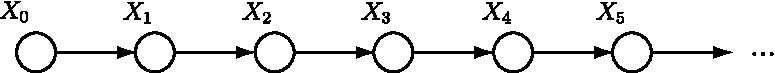
\includegraphics[width=\textwidth]{illus/mcdag.pdf}
\end{center}
And the variables $X_t$ can be scalars or vectors.  
\begin{itemize}
\item For most of the {\em examples} in this lecture, $X_t$ will be univariate.
\item When $X_t$ includes all the variables in an MCMC application, however, it is typically high-dimensional.
\end{itemize}



\newslide{A genetics example---the Wright-Fisher population}
Let $X_t$ denote the number of alleles of type $A$ in a Wright-Fisher population of size $N$ diploids.  Then:
\[
P(X_t=j|X_{t-1}=i) = \frac{2N!}{(2N-j)!j!} \biggl({\textstyle \frac{i}{2N}}\biggr)^j
\biggl({\textstyle \frac{2N-i}{2N}}\biggr)^{2N-j}
\]
\begin{itemize}
\item Important point:  conditional independence $\neq$ independence.  If you don't know $X_{t-1}$, then, of course $X_{t}$ depends on $X_{t-2}$
\begin{center}
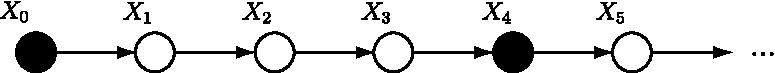
\includegraphics[width=.92\textwidth]{illus/mcdag_cond.pdf}
\end{center}

\item NB: Do not think that MCMC is useful in genetics because the problems in genetics involve Markov chains.  The Markov chain underlying Markov chain Monte Carlo and any Markov chains involved in a statistical genetics model may be quite distinct entities.  
\end{itemize}
   

\newslide{Transition Probability Matrices}
We can write down the transition probabilities from all values of $X_t$ to all values of $X_{t+1}$ in a matrix:  {\small
\[
	\bordermatrix{
  \nearrow &0   &   1&   2  & \cdots & 2N \cr
 0 &
	P(0\rightarrow 0) &
	 P(0\rightarrow 1) &
	 	 P(0\rightarrow 2) &
		 	\cdots &
			 	  P(0\rightarrow 2N) \cr
 1 &
	P(1\rightarrow 0) &
	 P(1\rightarrow 1) &
	 	 P(1\rightarrow 2) &
		 	 \cdots &
			 	  P(1\rightarrow 2N) \cr
2 &
	P(2\rightarrow 0) &
	 P(2\rightarrow 1) &
	 	 P(2\rightarrow 2) &
		 	 \cdots &
			 	  P(1\rightarrow 2N) \cr
3 &
	P(3\rightarrow 0) &
	 P(3\rightarrow 1) &
	 	 P(3\rightarrow 2) &
		 	 \cdots &
			 	  P(3\rightarrow 2N) \cr
\vdots & \vdots & \vdots &\vdots &\ddots & \vdots \cr
2N &
	P(2N\rightarrow 0) &
	 P(2N\rightarrow 1) &
	 	 P(2N\rightarrow 2) &
		 	 \cdots &
			 	  P(2N\rightarrow 2N) \cr
}
\]
}

Here we use $P(i\rightarrow j)$ as a shorthand for $P(X_{t+1}=j|X_t=i)$.

Such {\sl transition probability matrices} form the basis for much of the classical analysis of Markov chains.

The above t.p.m. is a bit unwieldy for examples, so consider another simple model\ldots

\newslide{Random walk with scattering boundaries}

Imagine a random walk on the integers from 1 to 5.  From 1 or 5, the walk goes to any state with equal probability, and from the remaining states, the walk may take steps of size 0 or 1, but they are biased toward the center.  

For example, consider the t.p.m:

\[
	\mP = \bordermatrix{
	\nearrow & 1 & 2 & 3 & 4 & 5 \cr
	1 & .2 & .2 & .2 & .2 & .2 \cr 
	2 & .2 & .3 & .5 & 0 & 0 \cr 
	3 & 0 & .3 & .4 & .3 & 0 \cr 
	4 & 0 & 0 & .5 & .3 & .2 \cr 
	5 & .2 & .2 & .2 & .2 & .2
	}
\] 
\fbox{Computer Demo}

\newpage
Some things to note:
\begin{itemize}
\item The rows of $\mP$ sum to one---they are probabilities that must sum to one
\item The columns need not sum to one
\item Probabilities after one step can be computed by matrix multiplication.  \ie{} if:
$\bm{v_0} = (0,1,0,0,0)$, then the probabilities of being in states 1,2,\ldots,5 after one step of the chain are given by:
\[
\bm{v_0}\mP = \bm{v_1} = (.2,.3,.5,0,0)
\] 
\item Probabilities after two steps are:
\[
	\bm{v_1}\mP = (\bm{v_0}\mP)\mP = \bm{v_2}
\]
\item and probabilities after $n$ steps are
\[
\bm{v_n} = \bm{v_0}\mP^n
\]
Vectors $\bm{v_t}$ are taken to be row vectors.
\end{itemize}

\newslide{Limiting Distributions}
A class of Markov chains called {\em ergodic Markov chains}\footnote{Conditions conferring ergodicity will be discussed a little later.} have the property that 
\[
	\lim_{n\rightarrow\infty} \mP^n = \left(\begin{matrix}
	\bpi \\
	\bpi \\
	\vdots \\
	\bpi
\end{matrix}
\right)
\]
where $\bpi$ is (in this discrete case) a vector referred to as the {\em limiting distribution} of the ergodic Markov chain.

Take our random walk example:
{\small
	\[
		\mP^1 = \bordermatrix{
	\nearrow & 1 & 2 & 3 & 4 & 5 \cr
	1 & .2 & .2 & .2 & .2 & .2 \cr 
	2 & .2 & .3 & .5 & 0 & 0 \cr 
	3 & 0 & .3 & .4 & .3 & 0 \cr 
	4 & 0 & 0 & .5 & .3 & .2 \cr 
	5 & .2 & .2 & .2 & .2 & .2
	},~
	\mP^2 = \bordermatrix{
	\nearrow & 1 & 2 & 3 & 4 & 5 \cr
	1 & 0.12& 0.20& 0.36& 0.20& 0.12\cr 
	2 & 0.10& 0.28& 0.39& 0.19& 0.04\cr 
	3 & 0.06& 0.21& 
    0.46& 0.21& 0.06\cr
    4 &  0.04& 0.19& 0.39& 0.28& 0.10\cr 
    5 & 0.12& 0.20& 0.36& 0.20& 
    0.12
	}
	\]
	\[
	\mP^3 = \bordermatrix{
	\nearrow & 1 & 2 & 3 & 4 & 5 \cr
	1 & 0.088& 0.216& 0.392& 0.216& 0.088\cr 
	2 & 0.084& 0.229& 0.419& 0.202& 0.066\cr 
	3 & 0.066& 0.225& 0.418& 0.225& 0.066\cr 
	4 & 0.066& 0.202& 0.419& 0.229& 0.084\cr 
	5 & 0.088& 0.216& 0.392& 0.216& 0.088
	}
	\]
	
	\[
	\mP^5 = \bordermatrix{
	\nearrow & 1 & 2 & 3 & 4 & 5 \cr
	1 & 0.075 &  0.219 &  0.412 &  0.219 &  0.075 \cr
	2 & 0.074 &  0.220 &  0.415 & 0.218 &  0.073 \cr
	3 & 0.072 &  0.220 &  0.415 &  0.220 & 0.072 \cr
	4 & 0.073 &  0.218 &  0.415 &  0.220 &  0.074 \cr
	5 & 0.075 & 0.219 &  0.412 &  0.219 &  0.075 
	}
	\]
	
	\[
		\mP^\infty = \bordermatrix{
		\nearrow & 1 & 2 & 3 & 4 & 5 \cr
		1 & 0.07317 &  0.2195 &  0.4146 &  0.2195 &  0.07317 \cr  
		2&0.07317 &  0.2195 & 0.4146 &  0.2195 &  0.07317 \cr  
		3&0.07317 &  0.2195 &  0.4146 &  0.2195 & 0.07317 \cr  
		4&0.07317 &  0.2195 &  0.4146 &  0.2195 & 0.07317 \cr  
		5&0.07317 &  0.2195 &  0.4146 &  0.2195 &  0.07317
		}
	\]
}
\newpage
The limiting distribution in this case is
\[
	\bpi = (0.07317,~0.2195,~0.4146,~0.2195,~0.07317)
\]
\begin{itemize}
\item This means that if you start the chain from any of the five states, after a sufficient (and not very many in this case) number of steps, the probability that it will be found in any of the five states is essentially independent of its starting state.   

\item And, as we have already seen, it means that a ``time-average" over the chain converges to the limiting distribution. 

\item This second point is asserted by the weak law of large numbers for ergodic Markov chains which states that as the number of transitions (or steps) in an ergodic chain tends to infinity, the proportion of time the chain spends in a state tends to the limiting probability (\ie{} the appropriate component of $\bpi$) of that state\footnote{See Feller (1957)}.  

\item Thus, the states visited by an ergodic Markov chain may be used to compute a Monte Carlo average.  That is MCMC.
\end{itemize}

\newslide{The use of Markov Chains in Monte Carlo}
Monte Carlo with a Markov chain is pretty much the same as before:
\[
	\Exp[g(X)] = \frac{1}{n}\sum_{i=1}^n g(x^{(i)})
\]
except that now, the $x^{(i)}$ are states visited by a Markov chain having a limiting distribution that we wish to sample from. 

To implement this we must be able to construct an appropriate Markov chain. It must:
\begin{itemize}
\item be ergodic
\item have the right limiting distribution
\end{itemize} 
The remainder of the lecture shows how this is done.
\newpage
Important points to keep in mind:
\begin{enumerate}
\item If you can simulate {\em independent} samples, $x^{(1)},\ldots,x^{(n)}$, then, by all means, do so, and avoid MCMC if you can.
\item MCMC is most useful when the desired distribution to be sampled from is ``known only up to scale"---this means that the ``shape" of the distribution is known but its normalizing constant is not. 

A germane example of a distribution known only up to scale is the Bayesian posterior distribution of $\theta$ given data $Y$:
\[
	P(\theta|Y) = \frac{P(Y|\theta)P(\theta)}
		{\int_\theta P(Y|\theta)P(\theta)d\theta}
\] 
The denominator is a constant w.r.t. $\theta$.  It is the (typically unknown) normalizing constant.  However, the numerator is the joint density of the data $Y$ and the parameters $\theta$, which is often easy to compute. This is why MCMC is so useful to Bayesians.
\end{enumerate}

\newslide{Conditions ensuring a chain is ergodic}
A Markov chain is ergodic if:
\begin{enumerate}
\item {\sl It has no transient states}, \ie{} there are no states with an expected time to recurrence of $\infty$.  (This is not an issue with a finite state space).
\item {\sl It is irreducible}, \ie{} any state in the state space is reachable from any other state in the state space in a finite number of steps.
\item {\sl It is aperiodic}, \ie{} there exists no pair of states $i$ and $j$ such that the probability of reaching $j$ from $i$ is non-zero only if the number of steps is an integer multiple of some period $\tau$.  
\end{enumerate}
In discrete ``tree-like" state spaces, like pedigrees, reducibility can be an issue.  We take this up briefly in Session~10.


\newslide{General balance and the stationary distribution of a Markov chain}
Recall that we wish to construct an ergodic Markov chain with limiting distribution $\bpi$ equal to some distribution that we wish to sample from.  How might we do that?

One possibility is via a theorem which tells us about a property of $\bpi$:

{\sl If $\bpi$ is the limiting distribution of the ergodic Markov chain with t.p.m. $\mP$, then $\bpi$ is the unique stationary distribution that satisfies the general balance equation}
\[
	\bpi\mP = \bpi
\]

So, if we can find $\mP$ such that its unique stationary distribution is $\bpi$, and $\bpi$ is the distribution we wish to sample from, then we can use the chain defined by $\mP$ in MCMC.

This is, however, not a tractable approach in any problem of consequence.  In general it will be harder to (or just as difficult to) solve the general balance equation for $\bpi$ as it will be to draw independent samples from $\bpi$.

The main problem with solving the general balance equation is that all possible states in the distribution $\bpi$ must be considered simultaneously.  In most interesting problems, that number of states can be astronomically huge.  

The solution to this conundrum is to not try to solve the general balance equation directly, but, instead satisfy a ``locally-defined" balance condition (so that only two states in the state space need be considered simultaneously---rather than all of the states, simultaneously), AND do this in a way that ensures that general balance is satisfied.

This is quite a lovely thing.   

\newslide{Time-reversible Markov chains and detailed balance}
A special class of Markov chains are called ``time-reversible" Markov chains, because if you were to watch them running ``backward in time" they would look just the same as the chain running ``forward in time."  

The salient feature of such chains is that they satisfy the {\em detailed balance} (also called the {\em local balance}) condition.

Detailed balance with respect to $\pi$ between a pair of states $i$ and $j$, is satisfied  by a Markov chain with a stationary distribution $\bpi$, and a t.p.m $\mP$ having elements $P(x\rightarrow y)$ if  
\[
	\bpi(i)P(i\rightarrow j) = \bpi(j)P(j\rightarrow i).
\]
It is easy to show (by summing over all states $i$) that if detailed balance holds for every pair of states, then general balance is also satisfied.

\newslide{The Metropolis-Hastings Algorithm\footnote{Metropolis et al. (1953) and Hastings (1970).}}
The M-H algorithm provides a way to perform steps in a Markov chain that satisfy detailed balance. 

Imagine you wish to simulate a dependent sample from a target distribution $f$, and you are currently in state $i$.  The recipe is:
\begin{itemize}
\item Propose changing the state from state $i$ to a new state $j$.  Draw the state $j$ from a proposal distribution, $q(j|i)$ which may be conditional on $i$.
\item Accept and move to the new state $j$ with probability $R$ equal to the lesser of 1 or the {\em Hastings ratio}:
\[
	R(i\rightarrow j) = \min\left\{1,\frac{f(j)}{f(i)}\times\frac{q(i|j)}{q(j|i)}\right\}
\]
If you don't accept the move to state $j$, then stay where you are.
\end{itemize}




\newslide{M-H algorithm satisfies detailed balance}
\enlargethispage*{1000pt}
\vspace*{-1.5em}

To show the M-H algorithm satisfies detailed balance w.r.t. $f$, we write down $P(i\rightarrow  j)$ and $P(j\rightarrow i)$, for any $i$ and $j$, under the M-H algorithm.

$P(i\rightarrow j)$ is the product of the probabilities that we:
\begin{enumerate}
\item Propose going from $i$ to $j$. ~~~~~~$\mathrm{Prob} =  q(j|i)$
\item Accept that proposal.  ~~~~~~$\mathrm{Prob} = R(i\rightarrow j)=\min\{1,\frac{f(j)}{f(i)} \frac{q(i|j)}{q(j|i)}\} $
\end{enumerate}
And $P(j\rightarrow i)$ can be found similarly [using $R(j\rightarrow i)$].

Now, there are two possible cases:
\begin{description}
\item[Case I:~~] $f(j)q(i|j) > f(i)q(j|i)$,  in which case \\$R(i\rightarrow j)=1$ ~~~~~~and~~~~~~  
$R(j\rightarrow i)=\frac{f(i)}{f(j)} \frac{q(j|i)}{q(i|j)}$
\item[Case II:~~] $f(j)q(i|j) \leq f(i)q(j|i)$, in which case \\
$R(i\rightarrow j)=\frac{f(j)}{f(i)} \frac{q(i|j)}{q(j|i)}$ ~~~~~~and~~~~~~~ $R(j\rightarrow i)=1$. 
\end{description}




\newslide{M-H algorithm satisfies detailed balance (cont'd)}

So, $P(i\rightarrow j)$ and $P(j\rightarrow i)$ in those cases are:
\begin{description}
\item[Case I:~~] 
\[
P(i\rightarrow j) = q(j|i)~~~~~~~~~~~~~~~~ P(j\rightarrow i) = q(i|j) \times \frac{f(i)}{f(j)} \frac{q(j|i)}{q(i|j)}
\]
\item[Case II:~~]
\[
P(i\rightarrow j) = q(j|i) \times \frac{f(j)}{f(i)} \frac{q(i|j)}{q(j|i)}
~~~~~~~~~~~~~~~~
P(j\rightarrow i) = q(i|j)
\]
\end{description}
Both of which, with a little rearranging, yield:
\[
f(i)P(i\rightarrow j) = f(j)P(j\rightarrow i)
\]
which is the detailed balance equation.

\newslide{M-H algorithm example---beta distribution\footnote{Up to this point we have been dealing with discrete Markov chains.  The extension to continuous state spaces is straightforward.  In such cases, $\bpi$, $P$, $q$, and $f$ may be taken as probability density functions, rather than as probability mass functions, and the general balance equation is expressed by a collection of integrals rather than in terms of matrix multiplication: $\int_x\bpi(x)P(x\rightarrow y)dx = \bpi(y)\ \forall y$}}
Let $\theta$ be a variable with probability density function
\[
	f(\theta)\equiv\mathrm{Beta}(74,128) = \frac{\Gamma(74+128)}
	{\Gamma(74)\Gamma(128)} \theta^{73} (1-\theta)^{127}
\]	
Note that this is the posterior distribution of the frequency $\theta$ of allele $A$ at a locus, given a uniform prior, and a sample of 100 diploids in which are found 73 copies of allele $A$.

This distribution is known exactly, but for illustration, we will construct a Markov chain that has limiting distribution $f$, and sample from it.

\newslide{Step one: Choose a proposal distribution}
\enlargethispage*{1000pt}
One is free to choose any proposal distribution $q$.  The only property that it should satisfy is that if $q(i|j)>0$, then $q(j|i)$ should also be positive\footnote{And the proposal distributions used should fulfill irreducibility, \etc.  Clearly, also, some proposal distributions will work better than others. }.  Otherwise you end up wasting some time.  

We will choose a uniform density for $q$ with width $w$, centered on the current state $i$.  It looks like:
\begin{center}
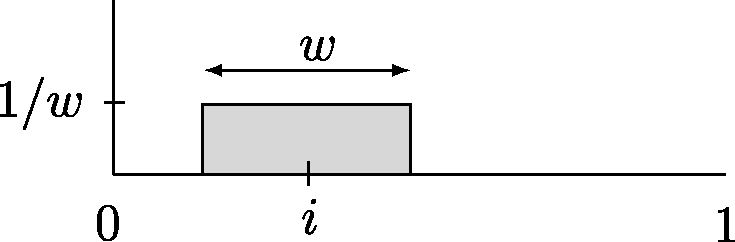
\includegraphics[width=.6\textwidth]{illus/propdist.pdf}
\end{center}
Thus, $q(i|j) = 1/w$ for all $i$ and $j$. (Note that if $j\geq1$ or $j\leq0$ then $f(j)=0$ and we reject the proposal immediately.)  

\newslide{Step two: Compute the Hastings Ratio}
\[
	\frac{f(j)}{f(i)}\frac{q(i|j)}{q(j|i)} = ~~~~~~~~~~~~~~~~~~~~~~~~~~~~~~~~~~~~~~~~~~~~~~~~~~~~~~~~~~~~~~~~~~~~~~~~~~~~~~~~~~~~~~~~~~~
\]

\[
 \frac{\Gamma(74+128)}
	{\Gamma(74)\Gamma(128)}\times
	\frac{\Gamma(74)\Gamma(128)}{\Gamma(74+128)}\times
	\frac{j^{73} (1-j)^{127}}{i^{73} (1-i)^{127}}\times
	\frac{1/w}{1/w}
\]

\[
= \left(\frac{j}{i}\right)^{73} 
\left(\frac{1-j}{1-i}\right)^{127}
\]
Notice that the normalizing constant cancels out.  (That {\em always} happens).  And, in this case, $q$ cancels out ({\em only because $q$ is symmetrical}).

\fbox{Computer Demo}

\newslide{Conclusions}
\begin{enumerate}
\item MCMC is just Monte Carlo with samples drawn from a Markov chain
\item The Markov chain in MCMC is constructed by concatenating moves together, each of which satisfies detailed balance
\item The rest of the module will explore methods for implementing MCMC in problems relevant to statistical genetics
\end{enumerate}



\end{document}